\section{Principal Component Analysis}
PCA is a tool used to find a low dimensional representation of a data set that represent as much variation as the complete data set.   The analysis finds uncorrelated variables named principal components from the dataset.  Using PCA would therefore also help lessen the change of "curse of dimensionality", and also improve the time needed to process the data. 

\begin{figure}[H]
\centering
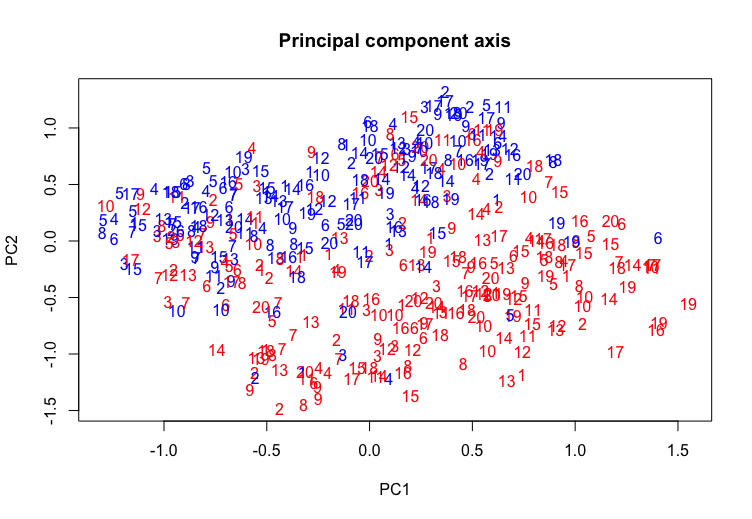
\includegraphics[width = \textwidth]{graphics/PCa-axis.png}
\caption{ red numbers indicated the axis of PC1 and the blue numbers determine the axis of PC2}
\label{fig:pca_vis}
\end{figure}

An illustration of the first two principal components of person dependent dataset can be seen in figure \ref{fig:pca_vis}. The axis shows how the data is distributed along both axis.  It shows that the PC1 axis has the greatest, as it can be seen from the variance of data aswell. 
\\
\\
As more PC gets included, will more of the variation of the dataset be exploited, and at the end completely resemble the the original data. The trick here is to find the right amount of PC which exploits the dataset as much as possible, and reduce the "unwanted" dimensions in the dataset. 

\begin{figure}[H]
\centering
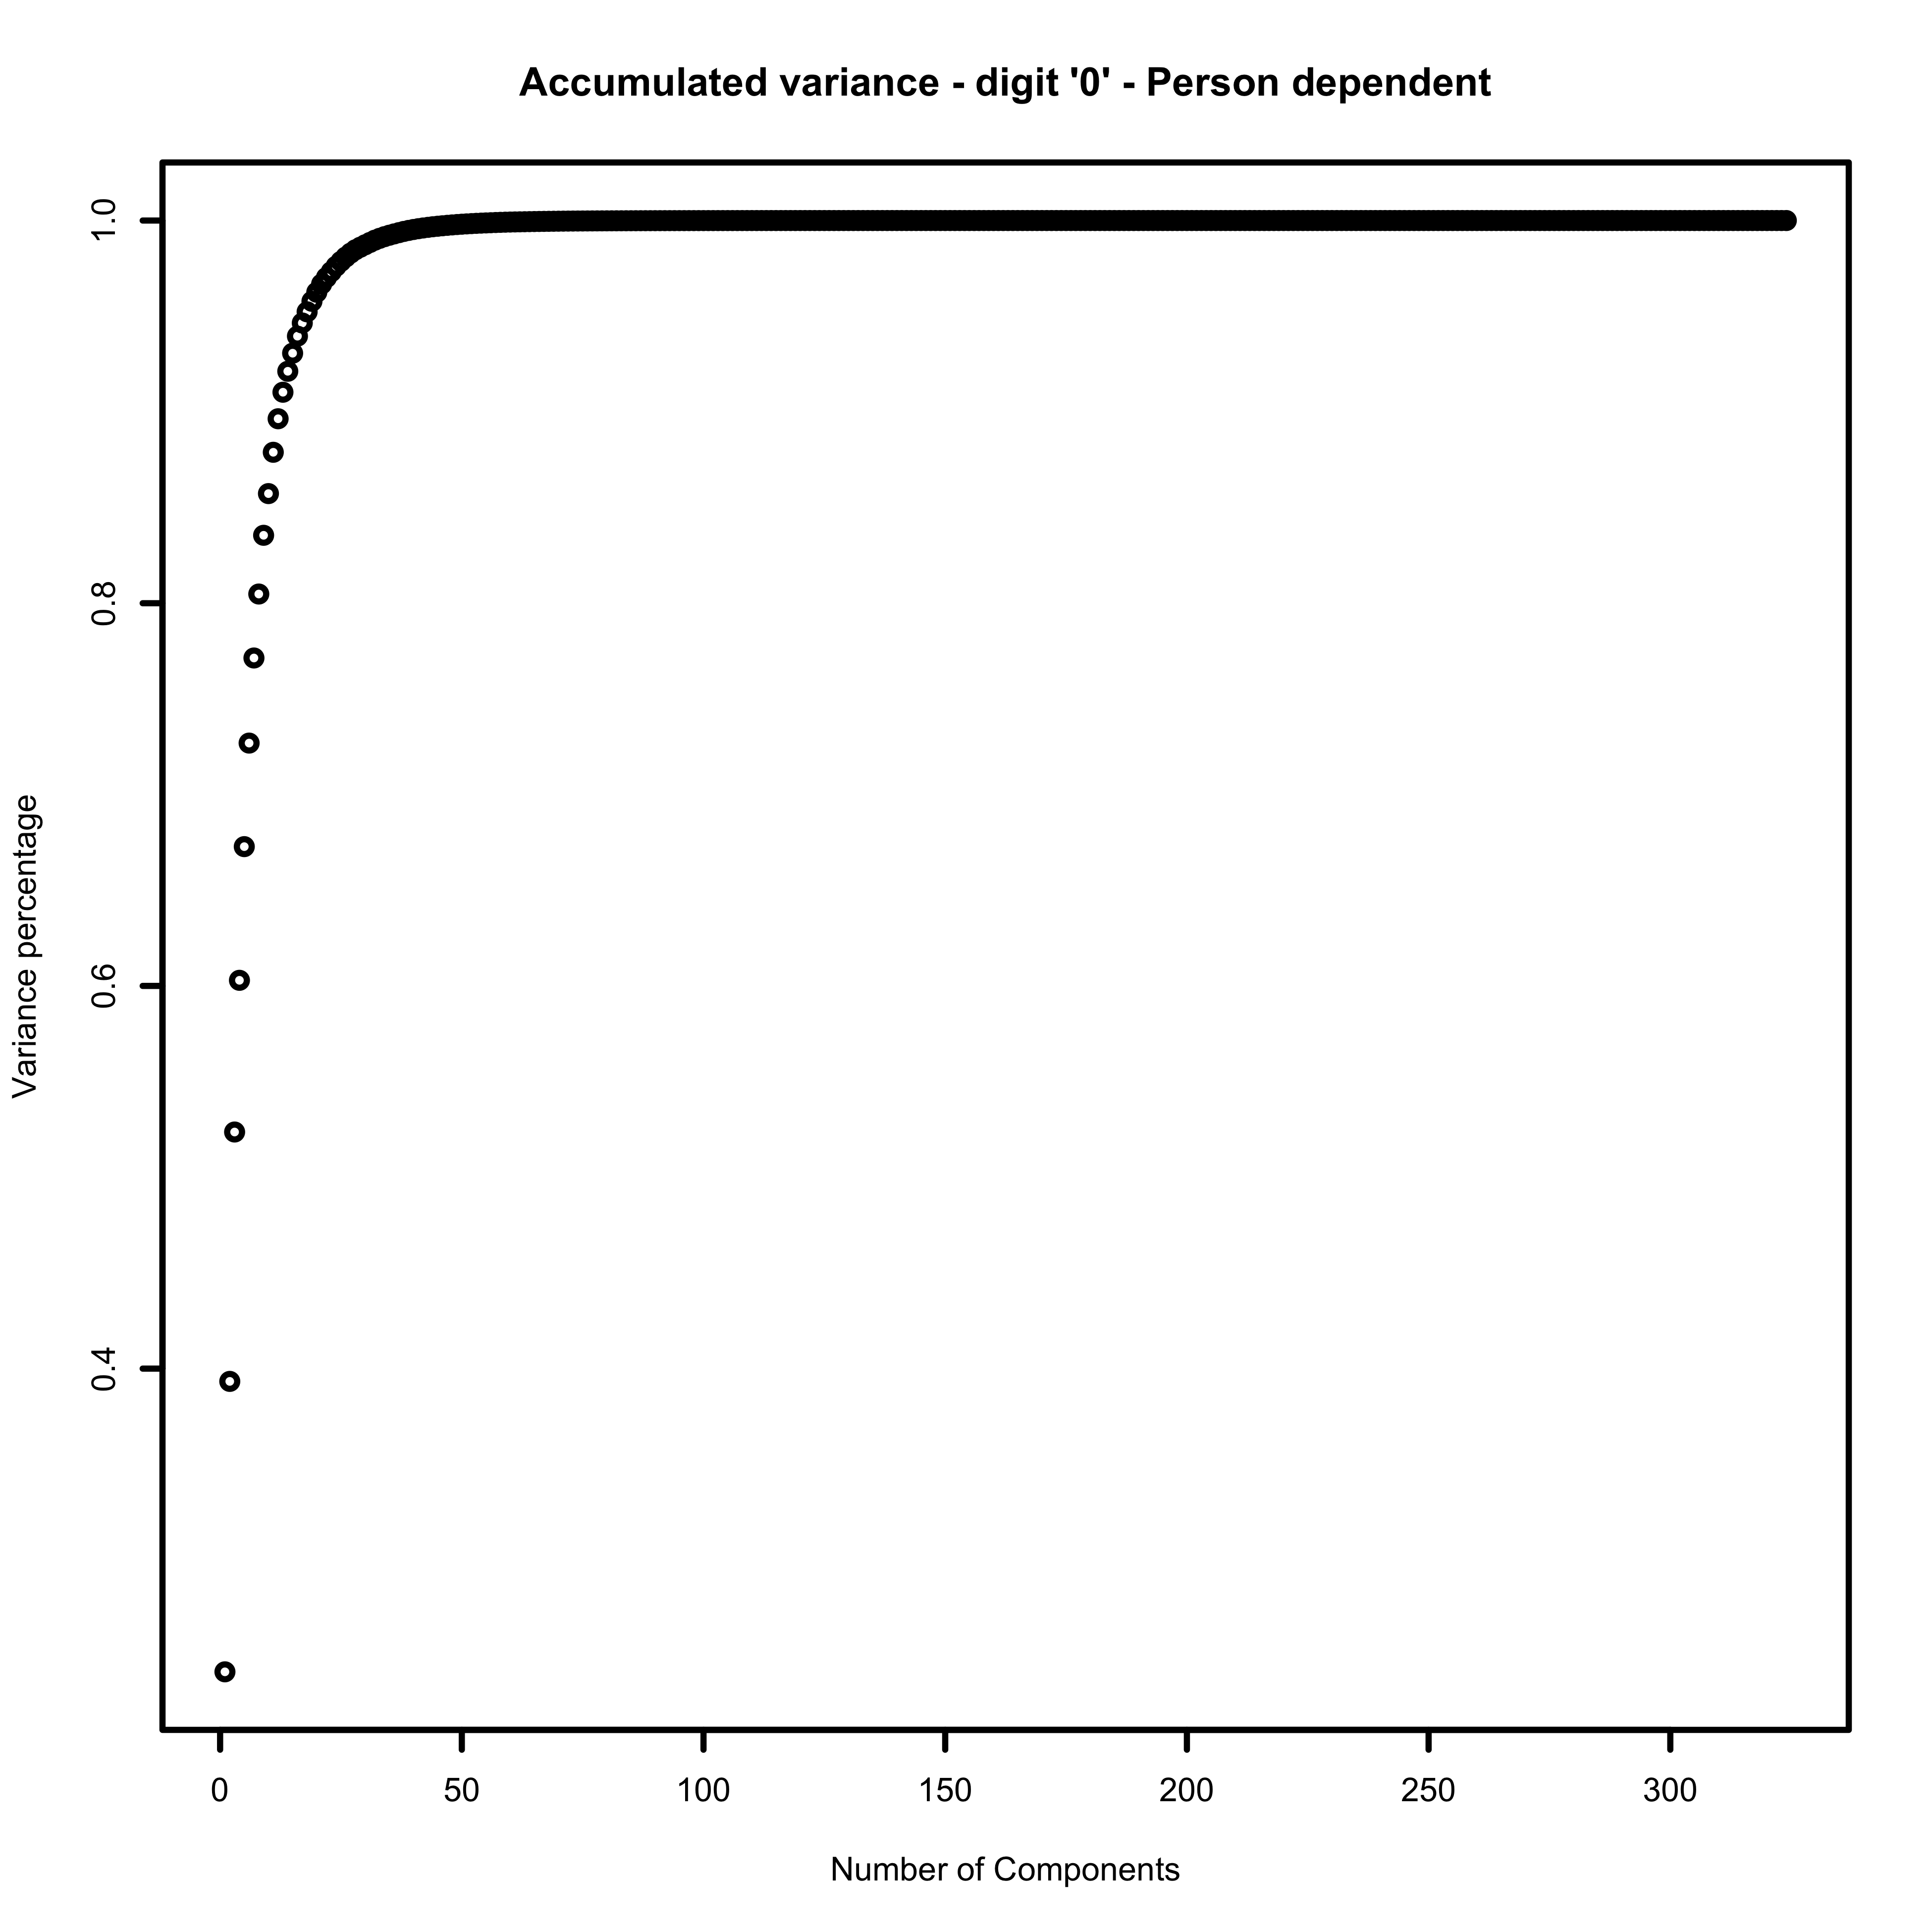
\includegraphics[width = 0.8\textwidth]{graphics/accumulated-2-1-person-dependent.png}
\caption{Plot showing the variance being accumulated for each component}
\label{fig:PCa_num_comp}
\end{figure}

As it can be seen in figure \ref{fig:PCa_num_comp} increased the accumalted variance strongly for the first principal components.  Using the elbow method one would be able to determine how many would be to determine how many would pc would fairly represent the dataset. 
\\
\\
\\
Using the PCA method were the dataset reduced into 4 sets  which represents 80\% , 90\%, 95\%, 99\% variances. The training was trained using a 10 - fold cross validation, which was repeated 10 times, and the accuracy mean was then computed. 

\begin{figure}[H]
\centering
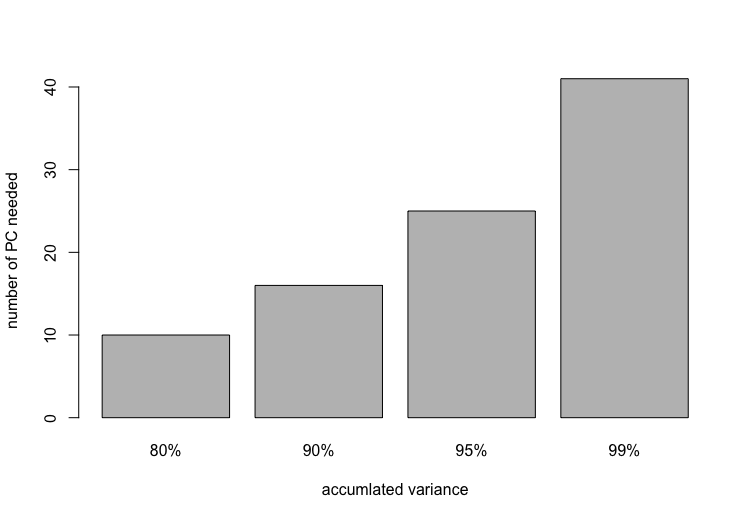
\includegraphics[width = \textwidth]{graphics/PCA_barplot.png}
\label{fig:pca_comp}
\caption{The number of components needed to achieve the desired variance}
\end{figure}

Using the PC were knn performed which resulted in this

\begin{figure}[H]
\centering
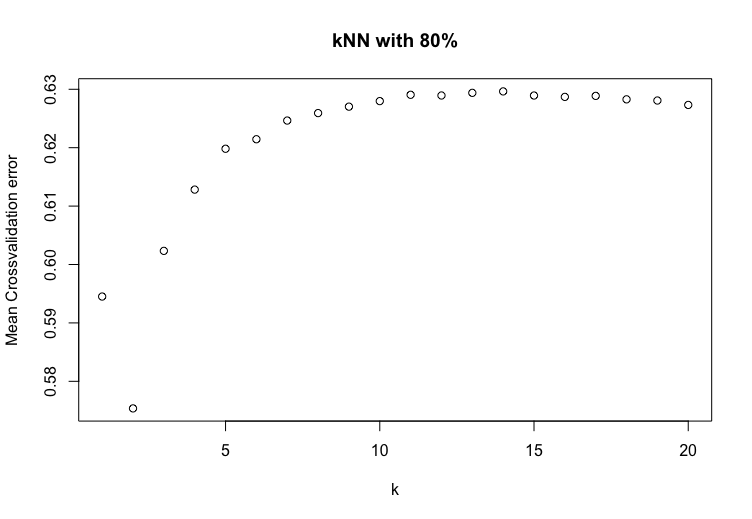
\includegraphics[width = \textwidth]{graphics/kNN_plot_80.png}
\label{fig:knnFit_80}
\end{figure}

\missingfigure{KnnFit Confusionmatrix}

\begin{figure}[H]
\centering
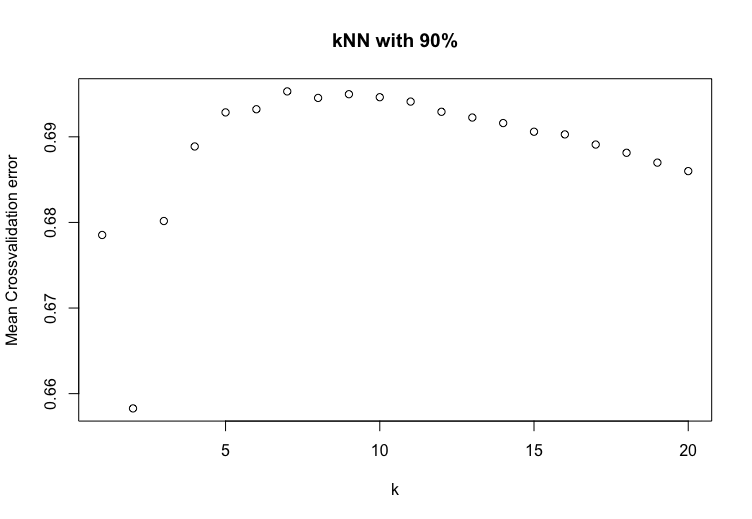
\includegraphics[width = \textwidth]{graphics/kNN_plot_90.png}
\label{fig:knnFit_90}
\end{figure}


\begin{figure}[H]
\centering
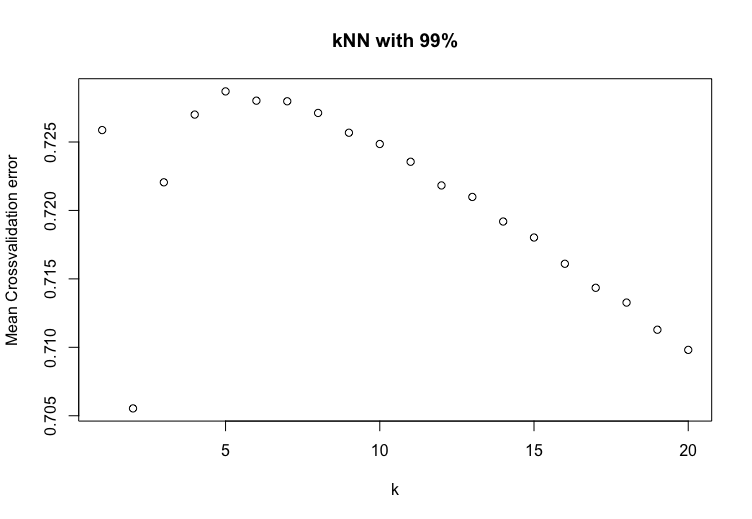
\includegraphics[width = \textwidth]{graphics/kNN_plot_99.png}
\label{fig:knnFit_99}
\end{figure}


\missingfigure{KnnFit plots}


\missingfigure{knnFit trainingTime}


\todo[inline]{prediction time.}